\section{Resultados e discussões}
%TODO: erros
\subsection{Sistema massa-mola}
%TODO: freq de oscilações
%TODO: const elástica da mola
%TODO: relação massa ~ freq
A partir dos dados extraídos do Tracker, resumidos nas \cref{molaG,molaP,2mola}, é notável observar o comportamento senoidal de todos os sistemas. É possível estimar a frequência do sistema massa-mola pela observação gráfica. Em \cref{molaG} a observação indica aproximadamente 1 oscilação por segundo. Enquanto em \cref{molaP} obtêm-se pouco mais de uma oscilação por segundo. E, em \cref{2mola} pouco menos de 1 oscilação por segundo.

No entanto, podemos também nos aproveitar do comportamento dos sistemas e obter uma equação para descrever cada um dos sistemas a partir da função horária da posição da massa considerando que tenha comportamento de um oscilador harmônico simples: 

\begin{align*}
    x(t) = A\cos(\omega t + \psi) + x_0
\end{align*}

Para o sistema com a mola maior e a massa de \qty{100}{\gram}, considerando os primeiros períodos, obtemos que os pontos de máximo e mínimo são: \(x(0) = \qty{-10}{cm}\), \(x(0,50) = \qty{20}{cm}\). Então, podemos extrair a função horária:

\begin{align*}
    x_{Gm}(t) = A\cos(\omega t + \psi) + x_{Gm0}\\
    x_{Gm}(0) = A + x_{Gm0} = \qty{20}{cm} \\
    x_{Gm}(1) = -A + x_{Gm0} = \qty{-10}{cm} \\
    \implies x_{Gm0} = \qty{5}{cm}\\
    \implies A = \qty{20}{cm} - \qty{5}{cm} = \qty{15}{cm}\\
    \text{Além de que:}\\
    x_{Gm}(0) \text{é mínimo} \implies \cos(\psi) = -1\\
    \implies \psi = \pi\\
    x_{Gm}(0,50) \text{é máximo} \implies \cos(0,5\omega + \pi) = 1\\
    \implies \omega = 2 \pi\\
    \implies x_{Gm}(t) = 15\cos(2\pi t + \pi) + 5\\
    \implies x_{Gm}(t) = -15\cos(2\pi t) + 5
\end{align*}

Esta é a fórmula deduzida para o sistema massa-mola apresentada em cinza na \cref{molaG}. É notável que a fórmula descreve bem o sistema nos períodos iniciais e começa a se comportar de maneira diferente ao longo de mais períodos. Esta divergência decorre de: (1) a dispersão de energia na forma de calor no sistema real, (2) a trepidação do sistema no eixo x, não oscilando perfeitamente na vertical, (3) a trepidação da câmera que registra o sistema, causando diferenças na altura absoluta da massa com relação a altura observada no software Tracker.

O mesmo processo pode ser utilizada para extrair a função horária da mola menor:

\begin{align*}
x_{pm}(t) = 8,1 \cos(\frac{\pi}{0,43}t) + 2,9
\end{align*}

    Que também apresenta divergências com relação aos dados extraídos do Tracker pela mesma justificativa que a mola maior, conforme observável na \cref{molaP}.
    Com as funções horárias é possível determinar a frequência dos osciladores:

\begin{align*}
    \nu = \frac{\omega}{2\pi}\\
    \nu_{pm} = \frac{\pi}{\num{0,43} \cdot 2\pi} = \num{1,16}\\ 
    \nu_{Gm} = \frac{2\pi}{2\pi} = 1
\end{align*}

Em que, \(\nu_{pm}\) é a frequência da mola pequena com massa de \qty{100}{g} e \(\nu_{Gm}\) é a mola grande com massa de \qty{100}{g}. Obtemos então, resultados compatíveis com a análise gráfica.

A partir das equações obtidas, é possível determinar a aceleração instantânea da massa a partir da segunda derivada das funções horárias. Em particular nos instantes \(t\) nos quais a aceleração é exatamente zero, sabemos que as forças atuando sobre o corpo estão em equilíbrio. Dessa forma, podemos determinar a constante elástica das molas:

\begin{align}
    \frac{d^2x_{pm}}{dt^2} = -43,81 \pi^2 \cos(\frac{\pi}{0,43}t)\\
    \frac{d^2x_{Gm}}{dt^2} = 60 \pi^2 \cos(2\pi t)\\ 
\end{align}

Sendo que a segunda derivada para a mola menor é 0 quando \(t = \qty{0,215}{s}\) ou \(t = \qty{0,645}{s}\) (se repetindo periodicamente para \(t + 2m\pi\) com \(m \in \mathbb{Z}\)) e a segunda derivada da mola maior é 0 quando \(t = \qty{0,25}{s}\) ou \(t = \qty{0,75}{s}\) seguindo as mesmas regras. Portanto, quando em equilíbrio de forças, \(x_{pm} = x_{pm}(0,215) = \qty{2,9}{cm}\) e \(x_{Gm} = \qty{-10}{cm}\).  

\begin{align*}
    \vec{F} = \vec{F_{el}} + \vec{F_{gm}} \\
    0 = -kx + gm\\
    k = \frac{gm}{x}\\
    k_{pm} = \qty{33.793103}{\gram\per\second\squared}\\
    k_{Gm} = \qty{19.6}{\gram\per\second\squared}
\end{align*}

\(\) 



\begin{figure}[H]
    \centering
    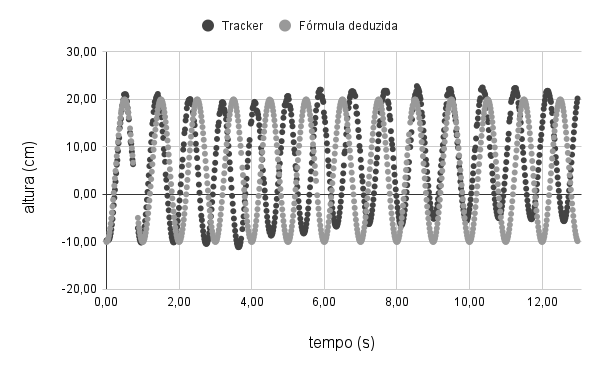
\includegraphics[width=.5\linewidth]{fig/molaG}
    \caption{Para mola grande com massa de \qty{100}{g}, gráfico de dispersão dos dados obtidos no Tracker em comparação aos valores nos mesmos instantes de tempo com a função horária deduzida}\label{molaG}
\end{figure}

\begin{figure}[H]
    \centering
    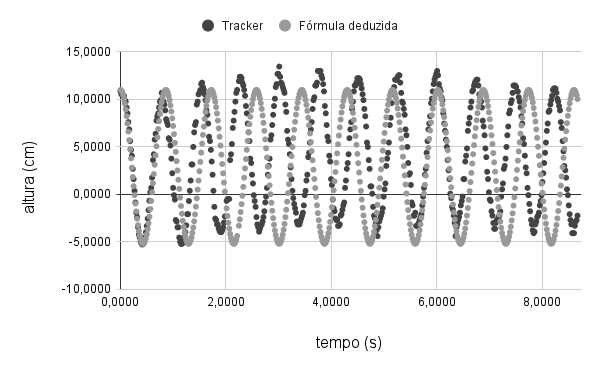
\includegraphics[width=.5\linewidth]{fig/molaP}
    \caption{Para mola pequena com massa de \qty{100}{g}, gráfico de dispersão dos dados obtidos no Tracker em comparação aos valores nos mesmos instantes de tempo com a função horária deduzida}\label{molaP}
\end{figure}
            
\subsection{Ondas}
%TODO: como o ocorre formação de nós;
%TODO: qual a diff entre esfera que vibra e e as molas?

    
